
\begin{frame}[fragile]{Clase: MainActivity\_Demo18}

\begin{itemize}
    \item Es la actividad principal de la aplicación.
    \item Controla la interacción entre la interfaz y la lógica del juego.
\end{itemize}


\textbf{Componentes principales:}
\begin{itemize}
    \item \textbf{TicTacToeView:} Vista personalizada (probablemente basada en SurfaceView) para el juego.
    \item \textbf{Button (B1):} Botón para reiniciar el juego.
\end{itemize}


\textbf{Funcionamiento:}
\begin{itemize}
    \item En \texttt{onCreate()}:
    \begin{itemize}
        \item Se carga el layout con \texttt{setContentView()}.
        \item Se inicializa el botón con \texttt{findViewById()}.
        \item Se asigna un \texttt{OnClickListener}.
    \end{itemize}
    \item Al presionar el botón:
    \begin{itemize}
        \item Se invoca \texttt{resetGame()} en la vista.
        \item Se reinicia el estado del juego (tablero, movimientos, etc.).
    \end{itemize}
\end{itemize}

\
\end{frame}



\begin{frame}[fragile]
\frametitle{Demo 18: Tic-Tac-Toe }
\begin{columns}
\column{0.80\linewidth}

\scriptsize
Del Repositorio Github:
\begin{itemize}
%\item Agregar la siguiente linea: \textit{implementation("com.github.PhilJay:MPAndroidChart:v3.1.0")}, al final de la seccion Dependencies del archivo Build.graddle.kts (Module: App).
%\item Agregar la siguiente linea: \textit{maven \{ url = uri(``https://jitpack.io'') \}}, al final de la seccion \textit{dependencyResolutionManagement } del archivo settings.graddle.kts.
\item Copiar el archivo \textit{MainActivity\_Demo18.java} (dentro del Folder códigosJAVA) al mismo directorio donde esta el MainActivity.java
\item Copiar los archivos \textit{TicTacToeView.java},  (dentro del Folder códigosJAVA) al mismo directorio donde esta el MainActivity.java
\item Copiar el archivo \textit{activity\_main\_demo18.xml} (dentro del Folder Carpeta\_layout) al mismo directorio donde esta el activity\_main.xml
\item Modificar dentro del archivo \textit{activity\_main\_demo18.xml} la cadena \textit{.com.example.a2026\_01\_holamundoandroid.TicTacToeView} por \textit{$<$SuPackage$>$.TicTacToeView}.
\item Modificar en el archivo \textit{AndroidManifest.xml} la cadena \textit{.MainActivity\_Demo17} por \textit{.MainActivity\_Demo18}.


%\item Ir a la linea 22 de archivo del archivo \textit{MainActivity\_Demo09.java}, poner el cursos en la palabra (en Rojo) \textit{documentfile}, presionar la combinación ALT+ENTER, y seleccionar de la lista desplegable la opcion ``Add dependency on ....''. Esto quitará el error y hara los ajustes necesarios. 
\end{itemize}

%\begin{block}{Demo \#09}
%Un App que permite escribir el contenido de un EditText a un archivo y cargar el contenido de cualquier archivo en el EditText
%\end{block}


\column{0.20\linewidth}

\begin{center}
 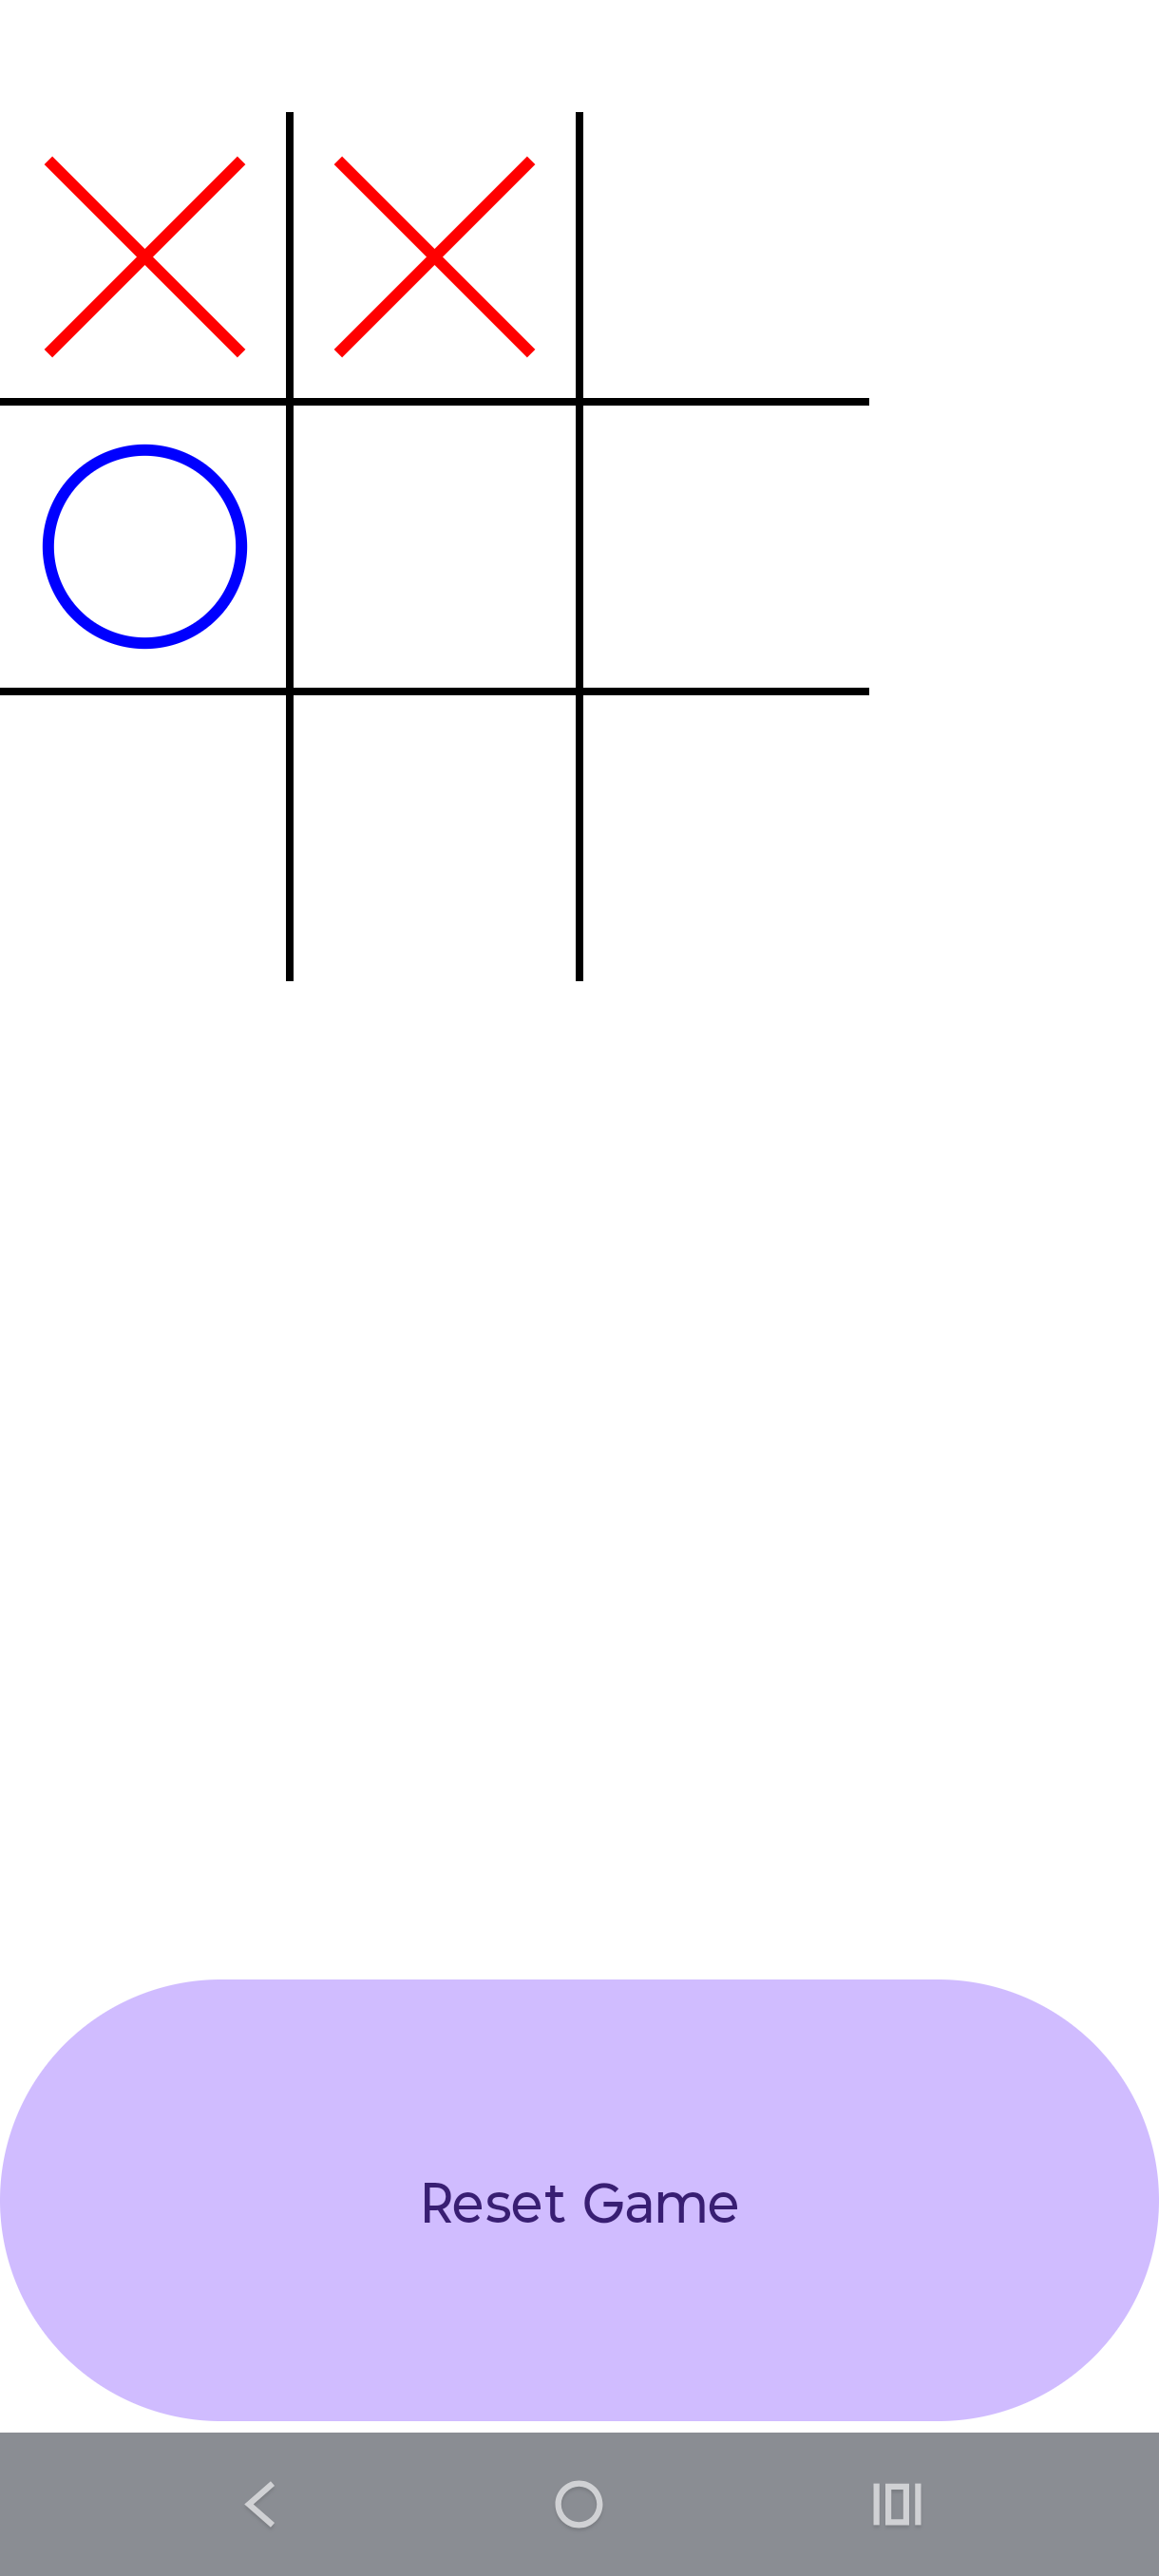
\includegraphics[width=0.98\textwidth]{02_TallerCBTis/figs/Demo18}
\end{center}

\end{columns}

\end{frame}

